\section*{Einleitung / Einführung ins Thema}
\addcontentsline{toc}{section}{Einleitung}
\Diskussionspunkt{- Kapitel muss noch fertiggestellt werden}\newline
\Diskussionspunkt{- Einführung, Problem, Aufgabenstellung, Struktur des Berichts, Ziel des Berichts}\newline
\Diskussionspunkt{- Kurze Zusammenfassung der Anforderungen (gruppiert nach Thema)}\newline

Die Wetterstation Arbon wurde 2004 als Lehrlingsarbeit des Berufsbildungszentrums Arbon auf Initiative der Technischen Gesellschaft Arbon (TGA) aufgebaut und in Betrieb genommen. Sie besteht aus mehreren Wettersensoren und einer Webcam, die auf einer Plattform auf dem See draussen montiert sind. Die Messwerte werden auf der Webseite\footnote{ \url{https://www.wetter-arbon.ch}}  der Wetterstation Arbon angezeigt.

\begin{figure}[h!]
	\centering
	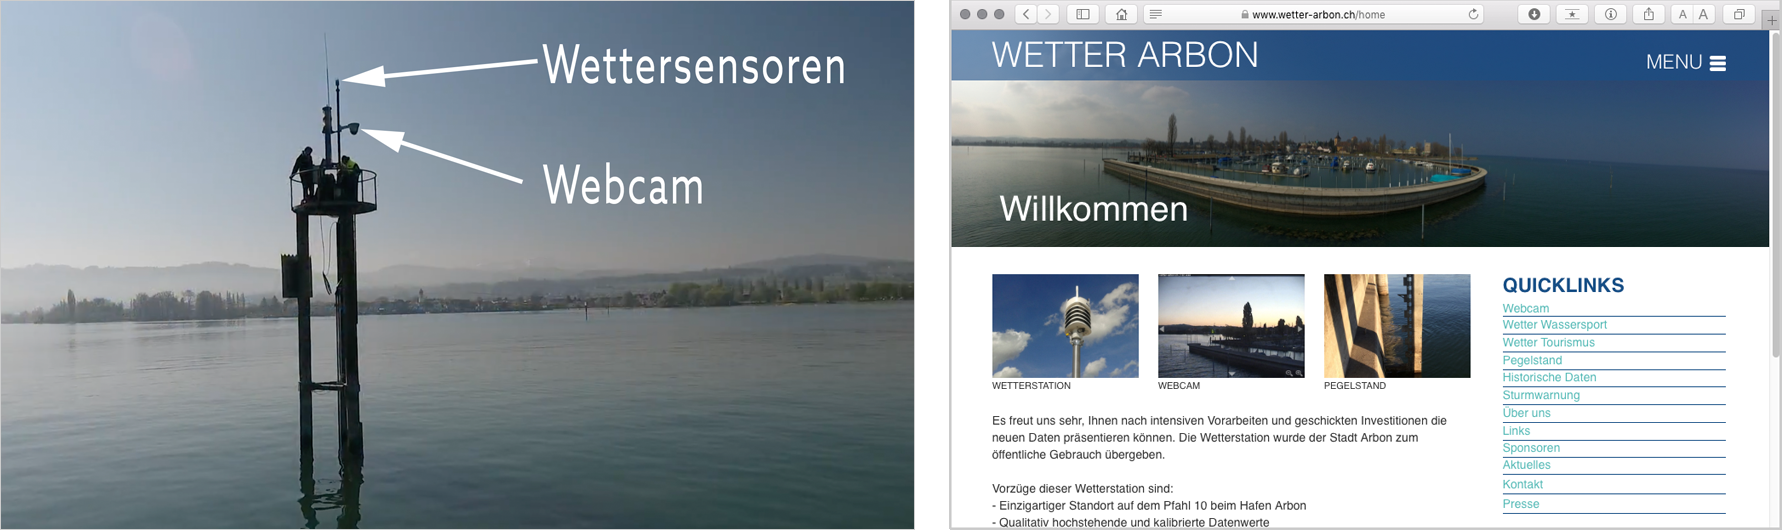
\includegraphics[width=1\linewidth]{img/kombi}
	\caption{Installation und Webseite der Wetterstation Arbon}
	\label{img:wetterstation}
\end{figure}

Die Bachelor-Arbeit hat das Ziel, die Wetterstation auf einen modernen, vollfunktionsfähigen Stand zu bringen. Die verschiedenen Arbeiten wurden in vier Blöcke zusammengefasst: Hardware, Webseite, Back end und Webcam. (vgl. Abb. \ref{img:module})

\vspace{5mm} %5mm vertical space

\begin{figure}[h!]
	\centering
	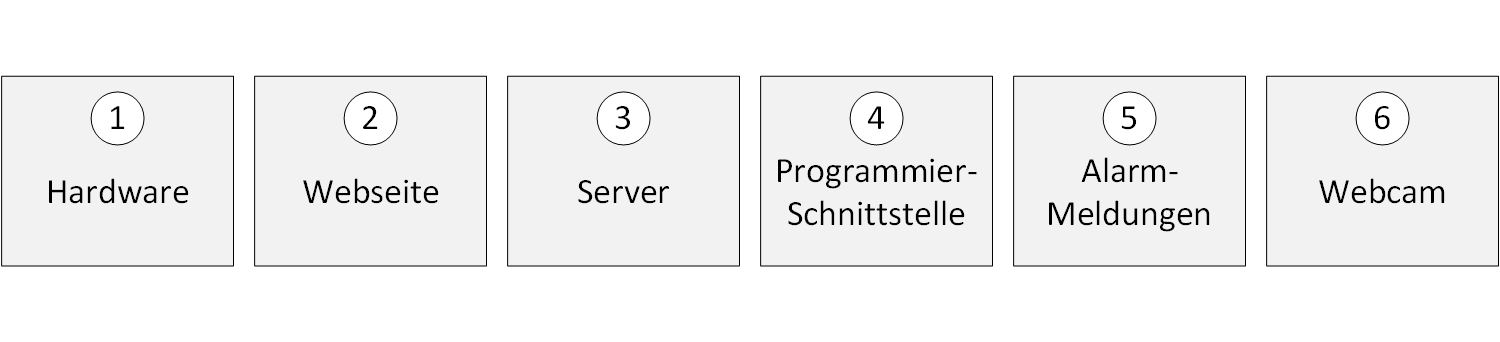
\includegraphics[width=0.8\linewidth]{img/module}
	\caption{Aufteilung in Arbeitsblöcke}
	\label{img:module}
\end{figure}


\newpage
